\documentclass[9pt]{beamer}
\usepackage{amsmath}
\usepackage{amssymb}
\usepackage[yyyymmdd]{datetime}
\renewcommand{\dateseparator}{ - }
\usepackage{graphicx}
\usepackage{tikz}
\usetikzlibrary{shapes.geometric, arrows}
\usetikzlibrary{positioning}
\definecolor{orange}{RGB}{235,113,37}
\definecolor{green}{RGB}{86,176,0}

\tikzstyle{IO} = [rectangle, rounded corners, minimum width=2cm, minimum height=1 cm , text centered, draw=black, fill=red!30]
\tikzstyle{process} = [rectangle, minimum width=2cm, minimum height=1 cm , text centered, draw=black, fill=orange]
\tikzstyle{adrianrules} = [rectangle, rounded corners, minimum width=2cm, minimum height=1 cm , text centered, draw=black, fill=green]
\tikzstyle{arrow} = [thick, ->, >=stealth]

\setbeamerfont{frametitle}{size=\huge}

\usetheme{default}
\usecolortheme{default}
\usefonttheme{professionalfonts}

\title{Synthesized PTZ}
\author{Adrian and Filip}

\begin{document}
\maketitle
\begin{frame}
	\frametitle{table of Contents}
	\tableofcontents
\end{frame}

\section{WHAAAAT?}
\begin{frame}
  %purpose
	ahubaboda!
\end{frame}

\section{implementation}

\begin{frame}
	\frametitle{implementation - overview}
	\begin{tikzpicture}[node distance=1.2cm]
		\node (input4) [IO] {User input};
		\node (input1) [IO, right of= input4, xshift=1.7cm] {\includegraphics[width=2cm]{../data/20150521_194353_C1D8.jpg}};
		\node (input2) [IO, right of= input1, xshift=1.3cm] {\includegraphics[width=2cm]{../data/20150521_194353_FD1E.jpg}};
		\node (input3) [IO, right of= input2, xshift=1.3cm] {\includegraphics[width=2cm]{../data/20150521_194353_49E3.jpg}};
		\node (SURF1) [process, below of= input1, yshift=-0.2cm] {Extract SURF features};
		\node (SURF2) [process, below of= input3, yshift=-0.2cm] {Extract SURF features};
		\node (Homo1) [process, below of= SURF1] {Homography to center image};
		\node (Homo2) [process, below of= SURF2] {Homography to center image};
		\node (PTZ) [process, below of= input4, yshift=-0.2cm] {PTZ matrix};
		\node (Trans) [process, below of= PTZ,yshift=-1.3cm] {Apply transformations};
		\node (Blend) [process, below of=Trans, yshift=-0.5cm] {Blend results};
		\node (Output) [IO, right of=Blend, xshift=4.5cm] {\includegraphics[width=7cm]{../results/images/res_stitch.PNG}};
		\draw [arrow] (input1) -- (SURF1);
		\draw [arrow] (input3) -- (SURF2);
		\draw [arrow] (input4) -- (PTZ);
		\draw [arrow] (SURF1) -- (Homo1);
		\draw [arrow] (SURF2) -- (Homo2);
		\draw [arrow] (PTZ)  -- (Trans);
		\draw [arrow] (Homo1)  |- (Trans);
		\draw [arrow] (Homo2)  |- (Trans);
		\draw [arrow] (input2) |- (Trans);
		\draw [arrow] (Trans) -- (Blend);
		\draw [arrow] (Blend) -- (Output);
	\end{tikzpicture}
\end{frame}

\subsection{Finding Homography}
\begin{frame}
	\frametitle{Finding Homography}
	\begin{tikzpicture}[node distance=1.2cm]
          \node (input1) [IO] {\includegraphics[width=5cm]{../data/20150521_194353_C1D8.jpg}};
          \node (input2) [IO, right of= input1, xshift=4.5cm] {\includegraphics[width=5cm]{../data/20150521_194353_FD1E.jpg}};
        \end{tikzpicture}
\end{frame}

\begin{frame}
	\frametitle{Finding Homography}
	\begin{tikzpicture}[node distance=1.2cm]
          \node (input1) [adrianrules] {\includegraphics[width=5cm]{../results/stitch_warped.jpg}};
          \node (input2) [adrianrules, right of= input1, xshift=4.5cm] {\includegraphics[width=5cm]{../results/rect_2.jpg}};
        \end{tikzpicture}
\end{frame}

\subsection{Pan, Tilt, Zoom camera}
\subsubsection{Camera rotation}

\begin{frame}
	\frametitle{Camera rotation}
	\begin{columns}
		\column{.5\textwidth}
		\begin{itemize}
			\item Rotations of camera in $\mathbb{R}^3$.
			\item $R_{pan}=\begin{pmatrix}
						1 & 0 & 0\\
						0 & cos(\theta) & -sin(\theta)\\
						0 & sin(\theta) & cos(\theta)
					\end{pmatrix}$
			\item $R_{tilt}=\begin{pmatrix}
						cos(\phi) & 0 & -sin(\phi)\\
						0 & 1 & 0 \\
						sin(\phi) & 0 & \cos(\phi)
					\end{pmatrix}$
			%\item Enter \emph{Homogenous coordinates}
			%\item $ \underset{\mathbb{R^2}}{(x,y)^T} \rightarrow \underset{\mathbb{P}^2}{(x,y,w)^T}$
			\item  Pan or tilt first?
			\item  tilt correction $\theta_{tiltCorr}$
		\end{itemize}
		\column{.42\textwidth}
		\includegraphics[width=\columnwidth]{../results/images/TiltPan.png}\\
		\includegraphics[width=\columnwidth]{../results/images/PanTilt.png}
	\end{columns}
\end{frame}

\subsubsection{Homogenous coordinates}
\begin{frame}
	\begin{columns}
		\column{.5\textwidth}
		\begin{itemize}
			\item Images are in $\mathbb{R}^2$, but rotations in $\mathbb{R}^3$.
			\item How to describe rotations in $\mathbb{R}^2$?\\
			\item Enter \emph{Homogeneous} Coordinates and \emph{Perspective transform}.
		\end{itemize}
			%Visa med block??
		\column{.5\textwidth}
		\begin{itemize}
			\item $\underset{\mathbb{R}^2}{(x,y)^T} \rightarrow \underset{\mathbb{P}^2}{(x,y,w)^T}$
			\item $H_{perspective} 
				\cdot 
				\begin{pmatrix} 
					x \\ 
					y \\
					w 
				\end{pmatrix}=
				\begin{pmatrix} 
					x' \\
					y' \\
					w'
				\end{pmatrix} 
				\overset{1/w'}{\rightarrow} 
				\qquad 
				\qquad 
				\qquad 
				\qquad 
				\qquad 
				\qquad 
				\overset{1/w'}{\rightarrow} 
				\underset{\mathbb{P}^2}{
					\begin{pmatrix} 
						x'/w' \\
						x'/w'\\
						w'/w'
					\end{pmatrix}}
					\rightarrow 
					\underset{\mathbb{R}^2}{
						\begin{pmatrix} 
							x'/w' \\
							y'/w' 
						\end{pmatrix}}$
		\end{itemize}
	\end{columns}
\end{frame}

\subsubsection{Perspective transform}
\begin{frame}
	\frametitle{Perspective transform}
	\begin{columns}
		\column{.5\textwidth}
		\begin{itemize}
			\item $H_{perspective}=KZR_{comp}K^{-1}$
			\item $R_{comp}=R_{Tilt}R_{pan}R_{tiltCorr}$
			\item $Z=\begin{pmatrix}
					Zoom_x   & 0 &0\\
					0   & Zoom_y &0\\
					0 & 0 & 1
				 \end{pmatrix}$
		\end{itemize}
		\column{.5\textwidth}
		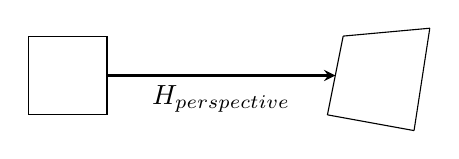
\begin{tikzpicture}
			\draw(0,0)|-(1,1);
			\draw(1,1)|-(0,0);
			\draw(3.8,0) -- (4.9,-.2);
			\draw(4.9,-.2) -- (5.1,1.1);
			\draw(5.1,1.1) -- (4,1);
			\draw(4,1) -- (3.8,0);
			\draw[arrow] (1,0.5) -- node[below]{$H_{perspective}$} (3.9,0.5);
		\end{tikzpicture}
	\end{columns}
\end{frame}

\subsection{Blending}
\begin{frame}
	\frametitle{Blending}
        \begin{tikzpicture}[node distance=1.2cm]
          \node (input1) [adrianrules, ] {\includegraphics[height=3cm]{../results/stitch_linear_1.jpg}};
          \node (input2) [adrianrules, right of= input1, xshift=4.5cm] {\includegraphics[height=3cm]{../results/stitch_linear_2.jpg}};
          \node (input3) [adrianrules, below of= input1, yshift=4.5cm] {\includegraphics[height=3cm]{../results/stitch_sigmoid_1.jpg}};
          \node (input4) [adrianrules, right of= input3, xshift=4.5cm] {\includegraphics[height=3cm]{../results/stitch_sigmoid_2.jpg}};
        \end{tikzpicture}
\end{frame}
\begin{frame}
	\frametitle{Blending}
        \begin{center}
          \begin{tikzpicture}[node distance=1.2cm]
            \node (input1) [adrianrules, ] {\includegraphics[height=3cm]{../results/stitch_linear_big.jpg}};
            \node (input2) [adrianrules, below of= input1, yshift=4.5cm] {\includegraphics[height=3cm]{../results/stitch_sigmoid_big.jpg}};
          \end{tikzpicture}
        \end{center}
\end{frame}

\section{Results}
\begin{frame}
	\frametitle{implementation}
	\begin{tikzpicture}[node distance=1.2cm]
		\node (input4) [IO] {User input};
		\node (input1) [IO, right of= input4, xshift=1.7cm] {\includegraphics[width=2cm]{../data/20150521_194353_C1D8.jpg}};
		\node (input2) [IO, right of= input1, xshift=1.3cm] {\includegraphics[width=2cm]{../data/20150521_194353_FD1E.jpg}};
		\node (input3) [IO, right of= input2, xshift=1.3cm] {\includegraphics[width=2cm]{../data/20150521_194353_49E3.jpg}};
		\node (SURF1) [process, below of= input1, yshift=-0.2cm] {Extract SURF features};
		\node (SURF2) [process, below of= input3, yshift=-0.2cm] {Extract SURF features};
		\node (Homo1) [process, below of= SURF1] {Homography to center image};
		\node (Homo2) [process, below of= SURF2] {Homography to center image};
		\node (PTZ) [process, below of= input4, yshift=-0.2cm] {PTZ matrix};
		\node (Trans) [process, below of= PTZ,yshift=-1.3cm] {Apply transformations};
		\node (Blend) [process, below of=Trans, yshift=-0.5cm] {Blend results};
		\node (Output) [IO, right of=Blend, xshift=4.5cm] {\includegraphics[width=7cm]{../results/images/res_stitch.PNG}};
		\draw [arrow] (input1) -- (SURF1);
		\draw [arrow] (input3) -- (SURF2);
		\draw [arrow] (input4) -- (PTZ);
		\draw [arrow] (SURF1) -- (Homo1);
		\draw [arrow] (SURF2) -- (Homo2);
		\draw [arrow] (PTZ)  -- (Trans);
		\draw [arrow] (Homo1)  |- (Trans);
		\draw [arrow] (Homo2)  |- (Trans);
		\draw [arrow] (input2) |- (Trans);
		\draw [arrow] (Trans) -- (Blend);
		\draw [arrow] (Blend) -- (Output);
	\end{tikzpicture}
\end{frame}

\begin{frame}
	\begin{center}
		{\Huge DEMO}
	\end{center}
\end{frame}

\begin{frame}
	\frametitle{PTZ-results}
	\begin{center}
		\begin{tikzpicture}[node distance=1.2cm]
			\node (Output) [IO] {\includegraphics[width=7cm]{../results/images/zoom_in.PNG}};
		\end{tikzpicture}
	\end{center}
\end{frame}


\begin{frame}
	\frametitle{PTZ-results}
	\begin{center}
		\begin{tikzpicture}[node distance=1.2cm]
			\node (Output) [IO] {\includegraphics[width=7cm]{../results/images/Pan.PNG}};
		\end{tikzpicture}
	\end{center}
\end{frame}


\begin{frame}
	\frametitle{PTZ-results}
	\begin{center}
		\begin{tikzpicture}[node distance=1.2cm]
			\node (Output) [IO] {\includegraphics[width=7cm]{../results/images/Tilt.PNG}};
		\end{tikzpicture}
	\end{center}
\end{frame}
%live ptz
%livekameror


\begin{frame}
  \begin{center}
    {\Huge Questions?}
  \end{center}
\end{frame}

\begin{frame}
	\frametitle{table of Contents}
	\tableofcontents
\end{frame}

\end{document}
